\section{RB-Methoden für lineare koerzive Probleme}
\label{sec-3}

\subsection{Primales RB-Problem}

\begin{defn}[Reduzierte Basis, RB-Räume]
	Sei $S_N = \set{\mu_1,\cdots,\mu_N} \subset \p$ Menge von Parametern mit (o.B.d.A.) linear unabhängigen Lösungen $\set{u(\mu_i)}_{i=1}^N$ von $\prob[\mu_i]$.
	Dann ist $X_N := \spn{\set{u(\mu_i)}_{i=1}^N}$ ein sog.\ \emph{Lagrange-RB-Raum}.\\
	Sei $\mu^0 \in \p$ und $u(\mu)$ Lösung von $\prob[\mu^0]$ $k$-mal diffbar in Umgebung von $\mu^0$.
	Dann ist
	\[
		X_{k,\mu^0} := \spn{\set{\partial_\sigma u(\mu^0) : \sigma \in \N_0^p, |\sigma| \leq k}}
	\]
	ein \emph{Taylor-RB-Raum}.
	Eine Basis $\Phi_N = \set{\phi_1,\cdots,\phi_N} \subseteq X$ eines RB-Raums ist eine \emph{reduzierte Basis}.
\end{defn}

\begin{bem} \beginwithlistbem
	\begin{itemize}
		\item $\Phi_N$ kann direkt aus Snapshots $u(\mu^i)$ oder, für numerische Stabilität (siehe \ref{sec-3.7}), auch orthonormiert sein.
		\item Wahl der Parameter $\set{\mu^i}$ ist entscheidend für Güte des RB-Modells:\\
			Hier: zufällige oder äquidistante Menge ausreichend\\
			Später: intelligente Wahl durch a-priori Analysis oder Greedy-Verfahren
		\item Es ex. auch andere Arten von RB-Räumen (Hermite, POD).
			Gemeinsam ist diesen die Konstruktion aus Snapshots von $u$ bzw.\ $\partial_\sigma u$.
		\item Andere MOR-Techniken: $\Phi_N$ kann auch komplett unabhängig von Snapshots auf andere Weise konstruiert werden: Balanced Truncation, Krylov-Räume, etc.\ (siehe z.B.\ Antoulas: Approximation of large scale dynamical systems, SIAM 2004)
	\end{itemize}
\end{bem}

\begin{defn}[Reduziertes Problem $\rprob$]
	Sei eine Instanz von $\prob$ gegeben und $X_N \subseteq X$ ein RB-Raum.
	Zu $\mu \in \p$ ist die RB-Lösung $u_N(\mu) \in X_N$ und Ausgabe $s_N(\mu) \in \R$ gesucht mit
	\begin{align*}
		a(u_N(\mu),v;\mu) &= f(v;\mu) &\forall v \in X_N\\
		s_N(\mu) &= l(u_N;\mu)
	\end{align*}
\end{defn}

\begin{bem} \beginwithlistbem
	\begin{itemize}
		\item Wir nennen obiges ``primal'' weil im Fall $f \neq l$ oder $a$ asymmetrisch, kann mit Hilfe eines geeigneten dualen Problems bessere Schätzung für $s$ erreicht werden.
		\item Obiges ist ``Ritz-Galerkin''-Projektion im Gegensatz zu ``Petrov-Galerkin''-Projektion, welches für nicht-koerzive Probleme notwendig ist. $\leadsto$ \ref{sec-4}
	\end{itemize}
\end{bem}

\begin{satz}[Galerkin-Projektion, Galerkin-Orthogonalität] \label{3.3}
	Sei $P_\mu : X \to X_N$ die orthogonale Projektion bzgl.\ Energieskalarprodukt $\dotp\pdot\pdot_\mu$, \emph{sei $a$ symmetrisch} und $u(\mu)$, $u_N(\mu)$ Lösung von $\prob$ bzw.\ $\rprob$.
	Dann:
	\begin{enumerate}
		\item $u_N(\mu) = P_\mu u(\mu)$ ``Galerkin-Projektion''
		\item $\dotp{e(\mu)}{v}_\mu = 0$ $\forall v \in X_N$, wobei $e(\mu) := u(\mu) - u_N(\mu)$
	\end{enumerate}

	\begin{proof}
		Nach Aufgabe 1/Blatt 1 ist $P_\mu$ wohldefiniert, denn $(X,\dotp\pdot\pdot_\mu)$ ist Hilbertraum und $X_N \subseteq X$ abgeschlossen weil endlichdimensional.
		Orthogonale Projektion des Fehlers ergibt
		\begin{align*}
			& & \dotp{P_\mu u(\mu) - u(\mu)}{\phi_i}_\mu &= 0 & \forall i = 1,\cdots,N &\\
			& \Leftrightarrow & a(P_\mu u(\mu) - u(\mu), \phi_i; \mu) &= 0 & \forall i = 1,\cdots,N &\\
			& \Leftrightarrow & a(P_\mu u(\mu), \phi_i; \mu) &= a(u(\mu),\phi_i;\mu) = f(\phi_i;\mu) & \forall i = 1,\cdots,N &
		\end{align*}
		\begin{enumerate}
			\item also ist $P_\mu u(\mu)$ Lösung von $\rprob$
			\item $e(\mu)$ ist also Projektions-Fehler, orthogonal nach Aufgabe 1/Blatt 1
		\end{enumerate}
	\end{proof}
\end{satz}

\begin{bem}
	Für $a$ nichtsymmetrisch gilt immer noch folgende ``Galerkin-Orthogonalität''
	\[
		a(u-u_N,v;\mu) = 0 \quad \forall v \in X_N
	\]
	(auch wenn $a$ kein Skalarprodukt)
\end{bem}

\begin{satz}[Existenz und Eideutigkeit für $\rprob$]
	Zu $\mu \in \p$ ex. eindeutige Lösung $u_N(\mu) \in X_N$ und RB-Ausgabe $s_n(\mu) \in \R$ von $\rprob$.
	Diese sind beschränkt
	\begin{align*}
		\norm{u_N(\mu)} &\leq \frac{\norm{f(\pdot;\mu)}_{X'}}{\alpha(\mu)} \leq \frac{\bar\gamma_f}{\bar\alpha}\\
		\norm{s_N(\mu)} &\leq \norm{l(\pdot;\mu)} \norm{u_N(\mu)} \leq \frac{\bar\gamma_l \bar\gamma_f}{\bar\alpha}
	\end{align*}

	\begin{proof}
		Weil $X_N \subset X$ ist $a(\pdot,\pdot;\mu)$ stetig und koerziv auf $X_N$.
		\begin{align*}
			\alpha_N(\mu) &:= \inf_{v \in X_N} \frac{a(v,v;\mu)}{\norm{v}^2} \geq \inf_{v \in X} \frac{a(v,v;\mu)}{\norm{v}^2} = \alpha(\mu) > 0\\
			\gamma_N(\mu) &:= \sup_{u,v \in X_N} \frac{a(u,v;\mu)}{\norm u \norm v} \leq \sup_{u,v \in X} \frac{a(u,v;\mu)}{\norm u \norm v} = \gamma(\mu) < \infty
		\end{align*}
		analog $f$, $l$ stetig auf $X_N$. Existenz, Eindeutigkeit und Schranken folgen also mit Lax-Milgram analog zu 2.8.
	\end{proof}
\end{satz}

\begin{kor}[Lipschitz-Stetigkeit]
	Seien $f$, $l$ gleichmäßig beschränkt und $a$, $f$, $l$ Lipschitz-stetig bzgl.\ $\mu$, dann sind auch $u_N(\mu)$, $s_N(\mu)$ Lipschitz-stetig bzgl.\ $\mu$ mit $L_u$, $L_s$ wie in 2.15.

	\begin{proof}
		Analog zu 2.15 / Übung.
	\end{proof}
\end{kor}

\begin{satz}[Diskrete RB-Probleme] \label{3.6}
	Sei $\Phi_N = \set{\phi_1,\cdots,\phi_N}$ eine reduzierte Basis für $X_N$.
	Für $\mu \in \p$,
	\begin{align*}
		A_N(\mu) &:= \seq{a(\phi_j,\phi_i;\mu)}_{i,j=1}^N & \in \R^{N \times N}\\
		\ubar l_N(\mu) &:= \seq{l(\phi_i;\mu)}_{i=1}^N & \in \R^N\\
		\ubar f_N(\mu) &:= \seq{f(\phi_i;\mu)}_{i=1}^N & \in \R^N
	\end{align*}
	und $\ubar u_N = \seq{u_{N,i}}_{i=1}^N \in \R^N$ als Lösung von
	\begin{equation}
		A_N(\mu) \ubar u_N = \ubar f_N(\mu)
		\label{eq:3.1}
	\end{equation}
	Dann ist $u_N(\mu) := \sum_{i=1}^N u_{N,i} \, \phi_i$ und $s_N(\mu) := \ubar l_N^\top(\mu) \ubar u_N$.

	\begin{proof}
		Einsetzen und Linearität zeigt, dass
		\[
			a \left(\sum u_{N,j} \, \phi_j, \phi_i; \mu \right) = \seq{A_N(\mu) \ubar u_N}_i = \seq{\ubar f_N}_i = f(\phi_i;\mu)
		\]
	\end{proof}
\end{satz}

\begin{satz}[Kondition bei ONB und Symmetrie]
	Falls $a(\pdot,\pdot;\mu)$ symmetrisch und $\Phi_N$ ist ONB, so ist Kondition von \eqref{eq:3.1} unabhängig von $N$ beschränkt
	\[
		\op{cond}_2(A_N) := \norm{A_N}_2 \norm{A_N^{-1}}_2 \leq \frac{\gamma(\mu)}{\alpha(\mu)}
	\]

	\begin{proof}
		Wegen Symmetrie gilt
		\begin{equation}
			\op{cond}_2(A_N) = \frac{|\lambda_\text{max}|}{|\lambda_\text{min}|}
			\label{eq:3.2}
		\end{equation}
		mit betragsmäßig größtem/kleinstem Eigenwert $\lambda_\text{max}$/$\lambda_\text{min}$ von $A_N(\mu)$.
		Sei $\ubar u_\text{max} = \seq{u_i}_{i=1}^N \in \R^N$ Eigenvektor zu $\lambda_\text{max}$ und
		\[
			u_\text{max} := \sum_{i=1}^N u_i \, \phi_i \quad \in X_N
		\]
		Dann gilt
		\begin{align*}
			\lambda_\text{max} \norm{\ubar u_\text{max}}^2 &= \lambda_\text{max} \ubar u_\text{max}^\top \ubar u_\text{max} = \ubar u_\text{max}^\top A_N \ubar u_\text{max}\\
			&= \sum_{i,j=1}^N u_i u_j \, a(\phi_j,\phi_i;\mu) = a\left(\sum_j u_j \phi_j, \sum_i u_i \phi_i; \mu\right)\\
			&= a(u_\text{max},u_\text{max};\mu) \leq \gamma(\mu) \norm{u_\text{max}}^2
		\end{align*}
		Wegen
		\[
			\norm{u_\text{max}}^2 = \dotp{\sum u_i \phi_i}{\sum u_j \phi_j} = \sum u_i u_j \dotp{\phi_i}{\phi_j} = \sum u_i^2 = \norm{\ubar u_\text{max}}^2
		\]
		folgt $|\lambda_\text{max}| \leq \gamma(\mu)$. Analog zeigt man $|\lambda_\text{min}| \geq \alpha(\mu)$ also folgt mit \eqref{eq:3.2} die Behauptung.
	\end{proof}
\end{satz}

\begin{bem}[Unterschied FEM zu RB]
	Es bezeichne $A_h(\mu) \in \R^{H \times H}$ die FEM Matrix (oder FV/FD).
	\begin{enumerate}
		\item Die RB-Matrix $A_N(\mu) \in \R^{H \times H}$ ist klein aber typischerweise vollbesetzt im Gegensatz zur großen aber dünnbesetzten Matrix $A_h$.
		\item Die Kondition von $A_N$ verschlechtert sich nicht mit wachsendem N (falls eine ONB verwendet wird), während die Konditionszahl von $A_h$ typischerweise polynomiell in $H$ wächst, also schlechter wird.
	\end{enumerate}
\end{bem}

\begin{satz}[Reproduktion von Lösungen] \label{3.8}
	Seien $u(\mu)$, $u_N(\mu)$ Lösungen von $\prob$ bzw.\ $\rprob$, $\ubar e_i \in \R^n$ $i$-ter Einheitsvektor
	\begin{enumerate}
		\item Falls $u(\mu) \in X_N \quad \Rightarrow \quad u_N(\mu) = u(\mu)$
		\item Falls $u(\mu) = \phi_i \in \Phi_N \quad \Rightarrow \quad \ubar u_N(\mu) = \ubar e_i \in \R^N$
	\end{enumerate}

	\begin{proof} \beginwithlistbew
		\begin{enumerate}
			\item Mit $u(\mu)$, $u_N(\mu) \in X_N \Rightarrow e := u(\mu) - u_N(\mu) \in X_N$.
				Wegen Galerkin-Orthogonalität ($a(e,v;\mu) = 0 \; \forall v \in X_N)$ und Koerzivität folgt:
				\[
					0 = a(e,e;\mu) \geq \underbrace{\alpha(\mu)}_{> 0} \underbrace{\norm{e}^2}_{\geq 0} \quad \Rightarrow \quad \norm{e} = 0 \Rightarrow e = 0 \Rightarrow u = u_N
				\]
			\item $u_N(\mu) = \phi_i$, nach i).
				Mit Eindeutigkeit der Basisexpansion folgt die Behauptung.
		\end{enumerate}
	\end{proof}
\end{satz}

\begin{bem} \beginwithlistbem
	\begin{itemize}
		\item Reproduktion von Lösungen ist grundlegende Konsistenzeigenschaft.
			Es gilt trivialerweise falls/sobald Fehlerschranken vorliegen, aber für komplexe RB-Probleme ohne Fehlerschranken ist obiges ein guter Test.
		\item Validierung für Programmcode: Wähle Basis aus Snapshots $\phi_i = u(\mu^i)$, $i=1,\dots,N$, ohne Orthonormierung, dann muss $\ubar u_N(\mu^i) = \ubar e_i \in \R^N$ ein Einheitsvektor sein.
	\end{itemize}
\end{bem}

\subsection{Fehleranalyse}

\begin{satz}[Céa, Beziehung zur Bestapproximation] \label{3.9}
	Für alle $\mu \in \p$ gilt
	\[
		\norm{u(\mu)-u_N(\mu)} \leq \frac{\gamma(\mu)}{\alpha(\mu)} \inf_{v \in X} \norm{u-v}
	\]

	\begin{proof}
		$\forall v \in X_N$ mit Stetigkeit und Koerzivität
		\begin{align*}
			\alpha \norm{u-u_N}^2 &\leq a(u-u_N,u-u_N) = a(u-u_N,u-v) + \underbrace{a(u-u_N,v-u_N)}_{= 0 \text{ (Galerkin-Orth.)}}\\
			&\leq \gamma(\mu) \norm{u-u_N} \norm{u-v}
		\end{align*}
		Division durch $\alpha$, $\norm{u-u_N}$ liefert
		\[
			\norm{u-u_N} \leq \frac{\gamma}{\alpha} \norm{u-v}
		\]
		also Behauptung durch Infimum-Bildung.
	\end{proof}
\end{satz}

\begin{bem} \beginwithlistbem
	\begin{enumerate}
		\item Ähnliche Bestapproximationsaussagen gelten auch für andere Interpolationstechniken, aber die zugehörige Lebesgue-Konstante divergiert meist mit wachsender Dimension $N$.
			Obiges ist konzeptioneller Vorteil von Galerkin-Projektion über anderen Interpolationstechniken, da $\frac{\gamma}{\alpha}$ unabhängig von $N$ beschränkt bleibt.
			``Quasi-Optimalität'' der Galerkin-Projektion/des RB-Ansatzes.
		\item Falls $a(\pdot,\pdot;\mu)$ zusätzlich symmetrisch ist, kann um eine ``Wurzel'' verbessert werden mittels Normäquivalenz \ref{2.5} und Bestapproximation der orthogonalen Projektion (Aufg. 1/Blatt 1)
			\begin{align*}
				\sqrt{\alpha} \norm{u-u_N} &\stackrel{\ref{2.5}}{\leq} \norm{u-u_N}_\mu = \norm{u-P_\mu u}_\mu = \inf_{v \in X_N} \norm{u-v}_\mu \stackrel{\ref{2.5}}{\leq} \sqrt{\gamma} \inf_{v \in X_N} \norm{u-v}\\
				\Rightarrow \; \norm{u-u_N} &\leq \sqrt{\frac \gamma \alpha} \inf_{v \in X_N} \norm{u-v}
			\end{align*}
		\item Implikation von \ref{3.9}: Wähle guten Approximationsraum $X_N$, so wird Galerkin-Projektion/RB-Approximation auch garantiert gut sein.
	\end{enumerate}
\end{bem}

\begin{satz}[Ausgabe und Bestapproximation] \label{3.10} \beginwithlist
	\begin{enumerate}
		\item Für alle $\mu \in \p$ gilt
			\[
				|s(\mu)-s_N(\mu)| \leq \norm{l(\pdot;\mu)}_{X'} \frac{\gamma(\mu)}{\alpha(\mu)} \inf_{v \in X_N} \norm{u-v}
			\]
		\item Für den sog.\ ``compliant'' Fall (d.h.\ $a(\pdot,\pdot;\mu)$ symmetrisch und $l = f$) gilt sogar
			\begin{align*}
				0 \leq s(\mu)-s_N(\mu) &= \norm{u-u_N}_\mu^2\\
				&= \inf_{v \in X_N} \norm{u-v}_\mu^2\\
				&\leq \gamma(\mu) \inf_{v \in X_N} \norm{u-v}^2
			\end{align*}
	\end{enumerate}

	\begin{proof} \beginwithlistbew
		\begin{enumerate}
			\item Klar mit Céa, Bestapproximation und Linearität
				\[
					|s(\mu)-s_N(\mu)| = |l(u)-l(u_N)| = |l(u-u_N)| \leq \norm l \norm{u-u_N} \leq \norm{l} \frac{\gamma}{\alpha} \inf_{v \in X_N} \norm{u-v}
				\]
			\item Wegen $a(\pdot,\pdot;\mu)$ symmetrisch gilt wie in voriger Bemerkung
				\begin{equation} \label{eq:3.3}
					\norm{u-u_N}_\mu = \norm{u-P_\mu u}_\mu = \inf_{v \in X_N} \norm{u-v}
				\end{equation}
				Damit
				\begin{align*}
					s(\mu) - s_N(\mu) &= l(u)-l(u_N) \stackrel{f=l}{=} f(u) - f(u_N) = f(u-u_N)\\
					&= a(u,u-u_N) - \underbrace{a(u_N,u-u_N)}_{=0 \text{ (Gal.-Orth./Symm.)}} = \norm{u-u_N}_\mu^2\\
					&\stackrel{\ref{3.3}}{=} \inf_{v \in X_N} \norm{u-v}_\mu^2\\
					&\stackrel{\ref{2.5}}{\leq} \gamma \inf_{v \in X_N} \norm{u-v}^2
				\end{align*}
				Also insbesondere $s-s_N = \norm{u-u_N}_\mu^2 \geq 0$.
		\end{enumerate}
	\end{proof}
\end{satz}

\begin{bem} \beginwithlistbem
	\begin{itemize}
		\item Im ``compliant'' Fall ist der Ausgabefehler i.A.\ sehr klein, da das Quadrat des RB-Fehlers eingeht.
		\item Im ``nicht-compliant'' Fall geht der RB-Fehler nur linear in die Schranke ein, das wird später durch primal-duale Technik verbessert.
		\item Aus ii) folgt nicht nur Fehlerschranke, sondern sogar Vorzeichen-Information, $s_N(\mu)$ ist untere Schranke für $s$.
	\end{itemize}
\end{bem}

\begin{kor}[Monotoner Fehlerabfall in Energienorm]
	Falls $a(\pdot,\pdot;\mu)$ symmetrisch, $\seq{X_N}_{N=1}^{N_\text{max}}$ Folge von RB-Räumen, mit $X_N \subseteq X_{N'}$, $\forall N \leq N'$ (``hierarchische Räume'') und für $\mu \in \p$ setze $e_{u,N} := u(\mu)-u_N(\mu)$, $e_{s,N} := s(\mu)-s_N(\mu)$.
	\begin{enumerate}
		\item Dann ist $\seq{\norm{e_{u,N}}_\mu}_{N=1}^{N_\text{max}}$ monoton fallend.
		\item Falls $l=f$ (also ``compliant'' Fall) ist $e_{s,N}$ monoton fallend.
	\end{enumerate}

	\begin{proof} \beginwithlistbew
		\begin{enumerate}
			\item Mit \eqref{eq:3.3} gilt für $N \leq N'$
				\[
					\norm{e_{u,N}}_\mu = \norm{u-u_N}_\mu \stackrel{\eqref{eq:3.3}}{=} \inf_{v \in X_N} \norm{u-v}_\mu \geq \inf_{v \in X_{N'}} \norm{u-v}_\mu \stackrel{\eqref{eq:3.3}}{=} \norm{e_{u,N'}}_\mu
				\]
			\item Mit Satz \ref{3.10} ii) gilt
				\[
					e_{s,N} = \norm{e_{u,N}}_\mu^2 \text{, also Behauptung folgt mit i)}
				\]
		\end{enumerate}
	\end{proof}
\end{kor}

\begin{bem} \beginwithlistbem
	\begin{itemize}
		\item ``Worst-case'' ist Stagnation des Fehlers (unrealistisch, jeder neue Basisvektor müsste orthogonal zum Fehler $e_N(\mu)$ sein).
			In Praxis ist bei geschickter Basiswahl und ``glatten'' Problemen exponentielle Konvergenz zu erwarten, siehe Basisgenerierung, §\ref{sec-3.4}.
		\item Monotonie gilt nicht notwendigerweise bezüglich anderen Normen trotz Normäquivalenz
			\[
				c \norm{e_{u,N}}_\mu \leq \norm{e_{u,N}} \leq C \norm{e_{u,N}}_\mu \text{, mit $c$, $C$ unabhängig von $N$}
			\]
			Fehlernorm $\norm{e_{u,N}}$ kann gelegentlich anwachsen, bleibt aber in einem ``Korridor'', welcher monoton fällt.
	\end{itemize}

	\begin{figure}[H]
		\centering\small
		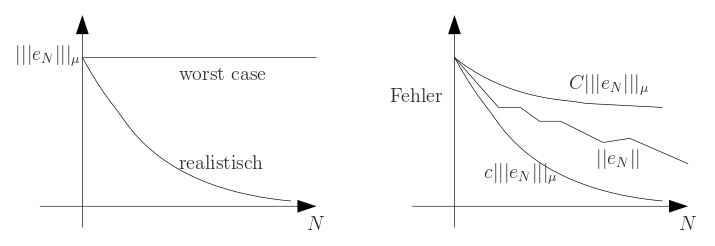
\includegraphics[width = 0.75 \textwidth]{Bilder/FehlerabfallEnergienorm.png}
		\caption{Fehlerabfall mit wachsender reduzierter Dimension.}{(aus B. Haasdonk, Reduzierte-Basis-Methoden, Skript zur Vorlesung SS 2011, Universität Stuttgart, IANS-Report 4/11, 2011.)}
		\label{fig:FehlerabfallEnergienorm}
	\end{figure}
\end{bem}

\begin{bem}[Gleichmäßige Konvergenz von Lagrange RB-Ansatz] \beginwithlistbem
	\begin{itemize}
		\item Sei $\p$ kompakt und $S_N := \set{\mu^1,\dots,\mu^N} \subset \p$, $N \in \N$, sodass die sog.\ Füll-Distanz (fill-distance) $h_N$ gegen 0 geht:
			\begin{align*}
				h_N &:= \sup_{\mu \in \p} \dist(\mu, S_N), \quad \dist(\mu,S_N) := \min_{\mu' \in S_N} \norm{\mu - \mu'}\\
				\lim_{N \to \infty} h_N &= 0
			\end{align*}
		\item Falls $u(\mu)$, $u_N(\mu)$ Lipschitz-stetig mit Lipschitz-Konstante $L_u$ unabhängig von $N$, so folgt für alle $N$, $\mu$ und ``nächstes'' $\mu^* := \arg\min_{\mu' \in S_N} \norm{\mu-\mu'}$:
			\begin{align*}
				\norm{u(\mu)-u_N(\mu)} &\leq \norm{u(\mu)-u(\mu^*)} + \norm{u(\mu^*)-u_N(\mu^*)} + \norm{u_N(\mu^*)-u_N(\mu)}\\
				&\leq L_u \underbrace{\norm{\mu-\mu^*}}_{\leq h_N} + 0 + L_u \underbrace{\norm{\mu - \mu^*}}_{\leq h_N} \leq 2 L_u h_N
			\end{align*}
		\item Also folgt uniforme Konvergenz
			\[
				\lim_{N \to \infty} \sup_{\mu \in \p} \norm{u(\mu)-u_N(\mu)} = 0
			\]
			\item Jedoch Konvergenzrate linear in $h_N$ ist nicht praktisch bedeutsam, weil $h_N$ sehr langsam mit $N$ abfällt, also muss $N$ sehr groß sein, um kleinen Fehler zu garantieren.
			\item Wir werden sehen, dass bei gleichmäßig koerziven Problemen und geschickter Wahl der $\mu^i$ sogar exponentielle Konvergenz erreicht wird.
	\end{itemize}
\end{bem}

\begin{lemma}[Fehler-Residuums-Beziehung] \label{3.12}
	Für $\mu \in \p$ definieren wir mittels der RB-Lösung $u_N$ das Residuum $r(\pdot;\mu) \in X'$ bzw.\ seinen Riesz-Repräsentanten $v_r(\mu) \in X$
	\[
		\dotp{v_r(\mu)}{v}_X := r(v;\mu) := f(v;\mu) - a(u_N(\mu),v;\mu) \quad \forall v \in X
	\]
	Dann erfüllt der Fehler $e(\mu) := u(\mu)-u_N(\mu)$
	\[
		a(e(\mu),v;\mu) = r(v;\mu) \quad \forall v \in X
	\]

	\begin{proof}
		$a(e(\mu),v;\mu) = \underbrace{a(u,v)}_{f(v)} - a(u_N,v) = r(v)$
	\end{proof}
\end{lemma}

\begin{bem} \beginwithlistbem
	\begin{itemize}
		\item Fehler erfüllt ``$\prob$ mit Residuum als rechte Seite''
		\item Insbesondere ist $r(v;\mu) = 0$ $\forall v \in X_N$ (wegen Galerkin-Orthogonalität)
		\item $r(\pdot;\mu) = 0 \quad \Rightarrow \quad e = 0$
	\end{itemize}
\end{bem}

\begin{satz}[A-posteriori Fehlerschätzer, absoluter Fehler] \label{3.13}
	Sei $\mu \in \p$, $u(\mu)$ bzw.\ $u_N(\mu)$ Lösung von $\prob$, $\rprob$ und $e=u-u_N$.
	Sei $\alpha_{LB}(\mu)$ eine untere Schranke für $\alpha(\mu)$ und $v_r \in X$ Riesz-Repräsentant von $r(\pdot;\mu)$ aus Lemma \ref{3.12}.
	Dann gelten folgende Schranken
	\begin{enumerate}
		\item Fehler in Energienorm
			\[
				\norm{e(\mu)}_\mu \leq \Delta_N^{en}(\mu) := \frac{\norm{v_r}}{\sqrt{\alpha_{LB}(\mu)}}
			\]
		\item Fehler in $X$-Norm $\norm\pdot$
			\[
				\norm{e(\mu)} \leq \Delta_N(\mu) := \frac{\norm{v_r}}{\alpha_{LB}(\mu)}
			\]
		\item Ausgabefehler
			\[
				|s(\mu)-s_N(\mu)| \leq \Delta_{N,s}(\mu) := \norm{l(\pdot;\mu)} \Delta_N(\mu)
			\]
	\end{enumerate}

	\begin{proof} \beginwithlistbew
		\begin{enumerate}
			\item Normäquivalenz \ref{2.5} impliziert
				\[
					\norm e \leq \frac{\norm{e}_\mu}{\sqrt{\alpha_{LB}(\mu)}}
				\]
				Damit folgt
				\[
					\norm{e}_\mu^2 = a_s(e,e) = a(e,e) = r(v) = \dotp{v_r}{e} \leq \norm{v_r} \norm{e} \leq \frac{\norm{v_r}}{\sqrt{\alpha_{LB}(\mu)}}
				\]
				Division durch $\norm{e}_\mu$ liefert die Behauptung i).
			\item Koerzivität liefert
				\[
					\alpha_{LB}(\mu) \norm{e}^2 \leq a(e,e) = r(e) = \dotp{v_r}{e} \leq \norm{v_r} \norm{e}
				\]
				Division durch $\alpha_{LB}$ und $\norm e$ liefert ii).
			\item Stetigkeit von $l$ liefert
				\[
					|s(\mu)-s_N(\mu)| = |l(u-u_N;\mu)| \leq \norm{l} \norm{u-u_N} \stackrel{ii)}{\leq} \norm{l} \Delta_N
				\]
		\end{enumerate}
	\end{proof}
\end{satz}

\begin{bem} \beginwithlistbem
	\begin{itemize}
		\item $\alpha_{LB}(\mu)$ soll eine \emph{schnell berechenbare} untere Schranke an $\alpha(\mu)$ sein, z.B.\ $\alpha_{LB}(\mu) := \bar \alpha$ falls $\bar \alpha$ bekannt, andere Möglichkeiten folgen später (``min $\Theta$'', ``SCM'').
		\item $\Delta_N$ ist also immer um Faktor $\sqrt{\alpha_{LB}(\mu)}$ schlechter.
		\item Beschränkung des Fehlers durch Residuums-Norm ist bekannte Technik aus FEM, um FEM-Lösung $u_h$ gegen Sobolev-Raum Lösung $u$ abzuschätzen.
			In diesem Fall ist $X$ $\infty$-dimensional und Residuums-Norm algorithmisch nicht berechenbar.
			In RB-Methoden wird $\norm{v_r}$ eine \emph{berechenbare} Größe sobald $X$ endlich-dimensional, z.B.\ FEM-Raum, ist.
			Für Residuum ist $u_N(\mu)$ erforderlich, daher sind Schranken ``\emph{a posteriori}''.
		\item Allgemeines Vorgehen (und alternative Begründung für ii)) zur Herleitung von Fehlerschranken: Zeige, dass Fehler $e$ erfüllt $\prob$ mit rechter Seite, genannt $r$ (Residuum), wende a-priori Stabilitätsaussage an:
			\[
				\norm{e} \leq \frac{\norm r}{\alpha(\mu)} \quad \text{z.B.\ Lax-Milgram}
			\]
			und erhalte berechenbare Größe durch Wahl $X=X_{FEM}$ und untere Schranke $\alpha_{LB}(\mu) \leq \alpha(\mu)$.
		\item Weil die Schranken beweisbare obere Schranken an Fehler darstellen, nennt man sie ``rigorose'' Fehlerschranken (vgl.\ ``zuverlässige'' Schätzer in FEM, bei denen jedoch die Konstante unbekannt ist).
		\item Fehlerschranken liefern eine Absicherung für RB-Methoden, ``certified'' RB-Methode, im Gegensatz zu vielen anderen Reduktionsmethoden (z.B.\ Krylov-Raum-Methoden).
		\item Ausgabefehler ist grob, indem $\Delta_N$ nur linear eingeht.
			Verbesserungen können für den ``compliant'' Fall oder mit primal-dual Techniken erreicht werden. ($\leadsto$ §\ref{sec-3.5})
	\end{itemize}
\end{bem}

\begin{kor}[Verschwindende Fehlerschranke] \label{3.14}
	Falls $u(\mu) = u_N(\mu)$ dann ist $\Delta_N(\mu) = \Delta_N^{en}(\mu) = \Delta_{N,s}(\mu) = 0$

	\begin{proof}
		\[
			0 = a(0,v;\mu) = a(e,v;\mu) = r(v;\mu)
		\]
		\[
			\Rightarrow r \equiv 0 \Rightarrow \norm{v_r} = 0 \Rightarrow \Delta_N = \Delta_N^{en} = \Delta_{N,s} = 0
		\]
	\end{proof}
\end{kor}

\begin{bem} \beginwithlistbem
	\begin{itemize}
		\item Dies ist initialer Wunsch an eine Fehlerschranke: diese soll verschwinden falls exakte Approximation vorliegt.
			Dies ist Grundlage dafür, dass der Faktor der Überschätzung endlich ist.
		\item Aussage ist trivial für \emph{effektive} Fehlerschätzer (sehen wir bald), aber in komplexen Problemen kann \ref{3.14} schon das maximal erreichbare sein.
		\item \ref{3.14} ist wieder sinnvoll um Programmcode zu validieren.
	\end{itemize}
\end{bem}

\begin{satz}[A-posteriori Fehlerschranken, relative Fehler] \label{3.15}
	Mit Bezeichnungen/Voraussetzungen aus \ref{3.13} und unter Annahme, dass alle Brüche im Folgenden wohldefiniert sind, gilt:
	\begin{enumerate}
		\item Für den relativen Fehler gilt in Energienorm:
			\[
				\frac{\norm{e(\mu)}_\mu}{\norm{u(\mu)}_\mu} \leq \Delta_N^{en,rel}(\mu) := 2 \frac{\norm{v_r}}{\sqrt{\alpha_{LB}(\mu)}} \cdot \frac{1}{\norm{u_N(\mu)}_\mu} \quad \text{falls} \quad \Delta_N^{en,rel} \leq 1
			\]
		\item Für den relativen Fehler gilt in $X$-Norm:
			\[
				\frac{\norm{e(\mu)}}{\norm{u(\mu)}} \leq \Delta_N^{rel}(\mu) := 2 \frac{\norm{v_r}}{\alpha_{LB}(\mu)} \cdot \frac{1}{\norm{u_N(\mu)}} \quad \text{falls} \quad \Delta_N^{rel} \leq 1
			\]
	\end{enumerate}

	\begin{proof} \beginwithlistbew
		\begin{enumerate}
			\item Falls $\Delta_N^{en,rel}(\mu) \leq 1$, so ist
				\begin{align*}
					\left| \frac{\norm{u}_\mu-\norm{u_N}_\mu}{\norm{u_N}_\mu} \right| &\stackrel{\Delta \text{-Ungl.}}{\leq} \frac{\norm{u-u_N}_\mu}{\norm{u_N}_\mu} = \frac{\norm{e}_\mu}{\norm{u_N}_\mu} \stackrel{\ref{3.13} \text{ i)}}{\leq} \frac{\norm{v_r}}{\sqrt{\alpha_{LB}(\mu)} \norm{u_N}_\mu}\\
					&= \frac 1 2 \Delta_N^{en,rel}(\mu) \leq \frac 1 2
				\end{align*}
				Falls $\norm{u_N}_\mu > \norm{u}_\mu$ gilt $\norm{u_N}_\mu-\norm{u}_\mu \leq \frac 1 2 \norm{u_N}_\mu$ also
				\[
					\frac 1 2 \norm{u_N}_\mu \leq \norm{u}_\mu \tag{$*$}
				\]
				Falls $\norm{u}_\mu \geq \norm{u_N}_\mu$, so ist ($*$) klar.
				Damit folgt
				\[
					\frac{\norm{e}_\mu}{\norm{u}_\mu} \stackrel{\ref{3.13} \text{ i)}}{\leq} \frac{\norm{v_r}}{\sqrt{\alpha_{LB}}} \cdot \frac{1}{\norm{u}_\mu} \stackrel{(*)}{\leq} \frac{\norm{v_r}}{\sqrt{\alpha_{LB}}} \cdot \frac{1}{\norm{u_N}_\mu} \cdot 2 = \Delta_N^{en,rel}(\mu)
				\]
			\item analog zu i).
		\end{enumerate}
	\end{proof}
\end{satz}

\begin{bem} \beginwithlistbem
	\begin{itemize}
		\item Analog folgt auch relativer Ausgabefehlerschätzer
			\[
				\frac{|s(\mu)-s_N(\mu)|}{|s(\mu)|} \leq \Delta_{N,s}^{rel}(\mu) := \frac{\norm{l(\pdot;\mu)} \cdot \Delta_N}{|s_N(\mu)|} \cdot 2 \quad \text{falls} \quad \Delta_{N,s}^{rel}(\mu) \leq 1
			\]
		\item Relative Fehlerschranken sind nur mit Zusatzbedingung ($\Delta_*^{rel} \leq 1$) gültig.
			Diese Bedingung ist jedoch konkret überprüfbar.
			Falls $\Delta_N^{rel}(\mu) > 1$, sollte der RB-Raum verbessert werden.
	\end{itemize}
\end{bem}

\begin{satz}[Effektivität der Fehlerschranken] \label{3.16}
	Mit Bezeichnungen aus \ref{3.13} sei $u(\mu) \neq u_N(\mu)$ und $\gamma_{UB}(\mu) < \infty$ eine obere Schranke an $\gamma(\mu)$.
	Dann sind die \emph{Effektivitäten} $\eta_N^{en}(\mu)$ und $\eta_N(\mu)$ definiert und beschränkt durch
	\begin{enumerate}
		\item
			\[
				\eta_N^{en}(\mu) := \frac{\Delta_N^{en}(\mu)}{\norm{e}_\mu} \leq \frac{\gamma_{UB}(\mu)}{\alpha_{LB}(\mu)}
			\]
			Falls $a(\pdot,\pdot;\mu)$ symmetrisch, gilt sogar $\eta_N^{en}(\mu) \leq \sqrt{\frac{\gamma_{UB}(\mu)}{\alpha_{LB}(\mu)}}$
		\item
			\[
				\eta_N(\mu) := \frac{\Delta_N(\mu)}{\norm{e}_\mu} \leq \frac{\gamma_{UB}(\mu)}{\alpha_{LB}(\mu)}
			\]
	\end{enumerate}

	\begin{proof} \beginwithlistbew
		\begin{enumerate}
			\setcounter{enumi}{1}
			\item $\norm{v_r}^2 = \dotp{v_r}{v_r} = r(v_r) = a(e,v_r) \leq \gamma_{UB}(\mu) \norm{e} \norm{v_r}$
				\begin{equation} \label{eq:3.4}
					\norm{v_r} \leq \gamma_{UB}(\mu) \norm{e}
				\end{equation}
				Damit
				\[
					\frac{\Delta_N(\mu)}{\norm{e}} = \frac{\norm{v_r}}{\alpha_{LB}} \cdot \frac{1}{\norm{e}} \stackrel{\eqref{eq:3.4}}{\leq} \frac{\gamma_{UB}}{\alpha_{LB}} \cdot \frac{\norm e}{\norm e}
				\]
			\setcounter{enumi}{0}
			\item
				\[
					\frac{\Delta_N^{en}(\mu)}{\norm{e}_\mu} = \frac{\norm{v_r}}{\sqrt{\alpha_{LB}}} \cdot \frac{1}{\underbrace{\norm{e}_\mu}_{\geq \sqrt{\alpha_{LB}} \cdot \norm{e}}} \leq \frac{\norm{v_r}}{\alpha_{LB}} \cdot \frac{1}{\norm{e}} \stackrel{\text{ii)}}{\leq} \frac{\gamma_{UB}}{\alpha_{LB}}
				\]
				Falls $a(\pdot,\pdot)$ symmetrisch, gilt wegen Normäquivalenz
				\[
					\norm{v_r}_\mu \leq \sqrt{\gamma_{UB}} \norm{v_r}
				\]
				und
				\[
					\norm{v_r}^2 = a(e,v_r) \stackrel{\text{CS}}{\leq} \norm{e}_\mu \norm{v_r}_\mu \quad \Rightarrow \quad \norm{v_r} \leq \norm{e}_\mu \cdot \sqrt{\gamma_{UB}}
				\]
				Damit
				\[
					\frac{\Delta_N^{en}(\mu)}{\norm{e}_\mu} = \frac{\norm{v_r}}{\sqrt{\alpha_{LB}}} \cdot \frac{1}{\norm{e}_\mu} \leq \frac{\norm{e}_\mu \cdot \sqrt{\gamma_{UB}}}{\sqrt{\alpha_{LB}} \cdot \norm{e}_\mu}
				\]
		\end{enumerate}
	\end{proof}
\end{satz}

\begin{bem} \beginwithlistbem
	\begin{itemize}
		\item Wir nennen $\Delta_N$, $\Delta_N^{en}$ daher ``effektive'' Fehlerschranken weil Faktor der Überschätzung höchstens $\frac{\gamma_{UB}}{\alpha_{LB}}$ beträgt.
		\item ``Rigorosität'' also äquivalent mit $\eta_N(\mu) \geq 1$.
		\item Für den Ausgabefehler $\Delta_{N,s}(\mu)$ ohne weitere Annahmen keine Effektivität beweisbar.
			Tatsächlich kann $\frac{\Delta_{N,s}}{|s-s_N|}$ beliebig groß oder nicht definiert sein, falls $\Delta_{N,s} \neq 0$, aber $s(\mu) = s_N(\mu)$:

			Wähle $X_N$ und $\mu$ so dass $u(\mu) \neq u_N(\mu)$, wird erreicht durch $u(\mu) \not\in X_N$
			\[
				\Rightarrow e(\mu) \neq 0 \Rightarrow \Delta_N \neq 0, \Delta_{N,s} \neq 0 \quad \text{falls} \quad l \neq 0
			\]
			Wähle $l(\pdot;\mu) \neq 0$, so dass $l(u-u_N;\mu) = 0$
			\[
				\Rightarrow s(\mu)-s_N(\mu) = l(u-u_N;\mu) = 0
			\]
		\item Wir nennen die Fehlerschranken auch \emph{Fehlerschätzer} weil sie äquivalent zum Fehler sind.
			\[
				\norm{e} \leq \Delta_N \leq \eta_N \norm{e}
			\]
	\end{itemize}
\end{bem}

\begin{satz}[Effektivität, relative Fehlerschätzer]
	Für $\Delta_N^{rel}(\mu)$ aus \ref{3.15} ist Effektivität definiert und beschränkt durch
	\[
		\eta_N^{rel}(\mu) := \frac{\Delta_N^{rel}(\mu)}{\frac{\norm{e}}{\norm{u}}} \leq 3 \frac{\gamma_{UB}(\mu)}{\alpha_{LB}(\mu)} \quad \text{falls} \quad \Delta_N^{rel}(\mu) \leq 1
	\]

	\begin{proof}
		Wie in Beweis zu \ref{3.15} impliziert $\Delta_N^{rel} \leq 1$:
		\[
			\left| \frac{\norm{u}-\norm{u_N}}{\norm{u}} \right| \leq \frac 1 2
		\]
		Falls $\norm{u_N} \leq \norm{u}$ so gilt $\norm{u}-\norm{u_N} \leq \frac 1 2 \norm{u_N}$ also
		\[
			\norm{u} \leq \frac 3 2 \norm{u_N}
		\]
		Falls $\norm{u_N} > \norm{u}$, so ist ($*$) klar.
		Dann gilt
		\[
			\eta_N^{rel}(\mu) = \underbrace{\frac{2 \norm{v_r}}{\alpha_{LB}(\mu) \norm{u_N}}}_{\Delta_N^{rel}} \cdot \frac{1}{\frac{\norm e}{\norm u}} \stackrel{\eqref{eq:3.4}}{\leq} 2 \frac{\gamma_{UB} \norm{e}}{\alpha_{LB} \norm{e}} \cdot \frac{\norm{u}}{\norm{u_N}} \stackrel{(*)}{\leq} 3 \frac{\gamma_{UB}}{\alpha_{LB}}
		\]
	\end{proof}
\end{satz}

\begin{bem} \beginwithlistbem
	\begin{itemize}
		\item Ähnlich für $\Delta_N^{en,rel}$
		\item Verbesserung von Schranken und Effektivität durch Normwechsel.

			Wähle $\bar\mu \in \p$ und $\norm{u} := \norm{u}_{\bar\mu}$ als neue Norm auf $X$.
			Dann gilt für symmetrisches $a$: $\alpha(\bar\mu) = 1 = \gamma(\bar\mu)$ also Effektivitäten $\eta_N$, $\eta_N^{en} = 1$, Schätzer sind genau der echte Fehler.
			Dies lässt $u_N$ unberührt, liefert aber bessere Fehlerschätzung.
			Im Fall von Stetigkeit bzgl.\ $\mu$ kann auch in Umgebung von $\bar\mu$ gute Effektivität erwartet werden.
	\end{itemize}
\end{bem}

\begin{satz}[Ausgabefehlerschranke und Effektivität, compliant Fall]
	Sei $a(\pdot,\pdot;\mu)$ symmetrisch, $l=f$. Dann erhalte verbesserte Ausgabeschranke
	\[
		0 \leq s(\mu) - s_N(\mu) \leq \bar \Delta_{N,s}(\mu) := \frac{\norm{v_r}^2}{\alpha_{LB}}
	\]
	und Effektivität
	\[
		\bar\eta_{N,s}(\mu) := \frac{\bar\Delta_{N,s}(\mu)}{s(\mu)-s_N(\mu)} \leq \frac{\gamma_{UB}(\mu)}{\alpha_{LB}(\mu)}
	\]

	\begin{proof}
		Nach Satz \ref{3.10} ii) und \ref{3.13} gilt
		\[
			0 \stackrel{\ref{3.10}}{\leq} s(\mu)-s_N(\mu) = \norm{u-u_N}_\mu^2 = \norm{e}_\mu^2 \stackrel{\ref{3.13}}{\leq} \Delta_N^{en}(\mu)^2 = \bar\Delta_{N,s}(\mu)
		\]
		Für Effektivität gilt entsprechend mit \ref{3.16} i)
		\[
			\bar\eta_{N,s}(\mu) = \frac{\bar\Delta_{N,s}}{s(\mu)-s_N(\mu)} \stackrel{\ref{3.10}}{=} \frac{\Delta_N^{en}(\mu)^2}{\norm{u-u_N}_\mu^2} = \eta_N^{en}(\mu)^2 \stackrel{\ref{3.16}}{=} \sqrt{\frac{\gamma_{UB}}{\alpha_{LB}}}^2 = \frac{\gamma_{UB}}{\alpha_{LB}}
		\]
	\end{proof}
\end{satz}

\begin{bem}
	Analog kann man im compliant Fall eine relative Ausgabefehlerschranke und Effektivität beweisen.
	\[
		\frac{s(\mu)-s_N(\mu)}{s(\mu)} \leq \bar\Delta_{N,s}^{rel}(\mu) := \frac{\norm{v_r}^2}{\alpha_{LB} s_N(\mu)}
	\]
	und
	\[
		\bar\eta_{N,s}^{rel}(\mu) := \frac{\bar\Delta_{N,s}^{rel}}{\frac{s(\mu)-s_N(\mu)}{s(\mu)}} \leq 2 \frac{\gamma_{UB}(\mu)}{\alpha_{LB}(\mu)}
	\]
	falls $\bar\Delta_{N,s}^{rel}(\mu) \leq 1$.
\end{bem}

\begin{bem}[Zusammenfassende Relevanz der Fehlerschätzer] \beginwithlistbem
	\begin{itemize}
		\item Rigorose obere Schranke für tatsächlichen Fehler nicht nur ``Indikatoren'' wie bei FEM.
		\item Effektivität Faktor der Überschätzung des Fehlers ist klein und bleibt beschränkt.
			Insbesondere:
			\[
				e(\mu) = 0 \Rightarrow \Delta_N(\mu) = 0
			\]
			also ``a-posteriori'' exakte Approximation verifizierbar.
		\item Theoretische Untermauerung der i.A.\ empirischen Basiswahl.
		\item Unabhängig von Basiswahl sind Fehlerschätzer anwendbar, auch für nicht-Snapshot-Basen (z.B.\ Krylov-Unterräume, etc.).
		\item Effiziente Berechnung: Durch Offline-Online-Zerlegung ($\leadsto$ §\ref{sec-3.3}) ist neben reduzierter Simulation auch Fehlerschranken \& Effektivitätsschranken schnell berechenbar.
		\item Weitere Einsatzmöglichkeiten: Offline zur Basisgenerierung ($\leadsto$ §\ref{sec-3.4}) und Online zur adaptiven Dimensionswahl.
	\end{itemize}
\end{bem}

\subsubsection*{Numerische Beispiele}

\paragraph*{demos\_chapter3(1)} Thermischer Block aus Beispiel \ref{2.10}, $B_1 = B_2 = 2$; $N = 5$, $\dotp{\pdot}{\pdot}_X := \dotp{\pdot}{\pdot}_{H_0^1}$,
\[
	S_N = \{ 0.1, 0.5, 0.9, 1.4, 1.7 \} \times \{0.1\}^3 \subseteq \R^4
\]
Erkenntnisse:
\begin{itemize}
	\item Fehlerschätzer kann günstig für sehr feines Parametergitter berechnet werden, Fehler ist teuer zu berechnen, daher nur in wenigen Punkten.
	\item Fehler und Schätzer sind $0$ für Basisparameter (bestätigt \ref{3.8}, \ref{3.14}).
	\item Fehlerschätzer ist obere Schranke für Fehler gemäß \ref{3.13}.
	\item Für kleine Werte von $\mu_1$ größere Fehler $\Rightarrow$ gute Wahl von $S_N$ wird vermutlich (und später bewiesen) hier mehr Samples benötigen.
\end{itemize}

\paragraph*{demos\_chapter3(2)} Effektivitäten $\eta_N(\mu)$ und obere Schranke $\frac{\gamma}{\alpha} \leq \frac{\mu_{max}}{\mu_{min}}$.\\
Erkenntnisse:
\begin{itemize}
	\item Effektivitäten sind gut, nur etwa Faktor $10$ über Fehler.
	\item Obere Schranke für Effektivität gemäß \ref{3.16}.
	\item Effektivitäten sind undefiniert für Parametersamples $\mu \in S_N$ (Division durch Null).
\end{itemize}

\paragraph*{demos\_chapter3(3)} Fehlerkonvergenz bezüglich $N$.
\[
	B_1 = B_2 = 3, \quad \mu_1 \in [0.5,2], \quad \mu = (\mu_1,1,\dots,1) \in \R^9
\]
Lagrange-Basis mit Gram-Schmidt-Orthonormierung, $\{\mu_i\}_{i=1}^N$ äquidistant.
Erkenntnisse für Testfehler: (Maximierung über 100 zufällige Parameter)
\[
	S_{test} \subset \p, \quad |S_{test}| = 100
\]

\begin{itemize}
	\item Exponentielle Konvergenz für Fehler und Schätzer.
	\item Obere Schranke sehr gut.
	\item Numerische Ungenauigkeiten für Schätzer.
\end{itemize}

\subsection{Offline/Online-Zerlegung} \label{sec-3.3}

Bisher:
\begin{itemize}
	\item $\rprob$ niedrigdimensional, aber noch keine schnelle Berechnungsvorschrift.
	\item Um ``berechenbares'' Verfahren zu erhalten: Forderung $\dim X < \infty$ in diesem Kapitel.
	\item Für effiziente Berechnung ist separierbare Parameterabhängigkeit von $\prob$ essenziell.
\end{itemize}
Offline-Phase:
\begin{itemize}
	\item Typischerweise berechnungsintensiv, Komplexität polynomiell in $H := \dim X$
	\item Einmal durchgeführt.
	\item Berechnung \emph{hochdimensionaler} Daten: Snapshots, reduzierte Basis, Riesz-Repräsentanten. (``detailed\_data'' in RBmatlab)
	\item Projektion der hochdimensionalen Daten in \emph{parameterunabhängigen niedrigdimensionalen} Daten. (``reduced\_data'')
\end{itemize}
Online-Phase:
\begin{itemize}
	\item Schnelle Berechnung, Komplexität polynomiell in $N$, $Q_a$, $Q_f$, $Q_l$, \emph{unabhängig von $H$}.
	\item Typischerweise häufig ausgeführt für variierendes $\mu$.
	\item Assemblierung des reduzierten parametrischen Systems für $\rprob$.
	\item Lösen von $\rprob$.
	\item Berechnung von Fehlerschranken und Effektivität.
\end{itemize}

\subsubsection*{Komplexitätsbetrachtung der bisherigen Formulierung}
\begin{itemize}
	\item Mit $\dim X = H$ und dünnbesetzter Matrix für $\prob$ ist Lösung z.B.\ in $\O(H^2)$ erreichbar (z.B.\ $H$ Schritte eines iterativen Lösers mit $\O(H)$ Komplexität für Matrix-Vektor-Multiplikation dank Dünnbesetztheit).
	\item  $N \times N$ System für $\rprob$ ist vollbesetzt, also in $\O(N^3)$ lösbar, also $N << H$ erforderlich, um Gewinn zu bewirken.
	\item Genaue Betrachtung der Berechnung von $u_N(\mu)$:
		\begin{enumerate}[1.]
			\item $N$ Snapshots berechnen mittels $\prob$: $\O(N \cdot H^2)$
			\item $N^2$ Auswertungen von $a(\phi_i,\phi_j;\mu)$: $\O(N^2 \cdot H)$
			\item $N$ Auswertungen von $f(\phi_i; \mu)$: $\O(N \cdot H)$
			\item Lösen des $N \times N$ Systems für $\rprob$: $\O(N^3)$
		\end{enumerate}
	\item Wir haben noch keine Offline/Online-Zerlegung: 1. gehört zur Offline-Phase, 4. gehört zur Online-Phase, aber 2. und 3. können nicht in Offline-Phase berechnet werden (wegen Parameterabhängigkeit) und nicht in Online-Phase (wegen $H$-Abhängigkeit).\\
		$\rightarrow$ Zerlegung von 2. und 3. mittels separierbarer Parameterabhängigkeit
\end{itemize}

\begin{defn}[Notation für Zerlegung von $\prob$]
\label{3.19}
	Unter Annahme $H = \dim X < \infty$, $X = \spn \set{\psi_i}_{i=1}^H$, definiere Matrix
	\[
		K := \seq{\dotp{\psi_i}{\psi_j}}_{i,j=1}^H \in \R^{H \times H} \quad \text{``Gram'sche Matrix'' / ``Skalarprodukt-Matrix''}
	\]
	Mit separierbare Parameterabhängigkeit definiere Matrizen und Vektoren
	\begin{align*}
		A^q &:= \seq{a^q(\psi_j,\psi_i)}_{i,j=1}^H \in \R^{H \times H}, & q = 1,\dots,Q_a \\
		\ubar f^q &:= \seq{f^q(\psi_i)}_{i=1}^H \in \R^H, & q = 1,\dots,Q_f \\
		\ubar l^q &:= \seq{l^q(\psi_i)}_{i=1}^H \in \R^H, & q = 1,\dots,Q_l
	\end{align*}
\end{defn}

\begin{kor}[Lösung von $\prob$]
\label{3.20}
	Lösung von $\prob$ wird erhalten durch Assemblieren des vollen Systems
	\[
		A(\mu) = \sum_{q=1}^{Q_a} \Theta_a^q(\mu) \cdot A^q, \quad \ubar f(\mu) = \sum_{q=1}^{Q_f} \Theta_f^q(\mu) \ubar f^q, \quad \ubar l(\mu) = \sum_{q=1}^{Q_l} \Theta_l^q(\mu) \ubar l^q
	\]
	und Lösen von $A(\mu) \ubar u(\mu) = \ubar f(\mu)$ nach $\ubar u(\mu) = \seq{u_i}_{i=1}^H \in \R^H$ und
	\[
		u(\mu) = \sum_{i=1}^H u_i \phi_i \in X, \quad s(\mu) = \ubar l^T(\mu) \cdot \ubar u(\mu)
	\]

	\begin{proof}
		Klar mit Definitionen.
	\end{proof}
\end{kor}

\begin{bem} \beginwithlistbem
	\begin{itemize}
		\item Das Vorliegen der $A^q$, $\ubar f^q$, $\ubar l^q$ ist nicht trivial im Fall von ``fremden'' Diskretisierungspaketen und stellt wesentliche Schwierigkeit in breiter praktischer Anwendung dar.
			Motivation für Eigenentwicklung von Diskretisierungscode.
		\item Sinn von Matrix $K$ ist Berechnung von Skalarprodukten und Normen, z.B.\ für
			\[
				u = \sum u_i \psi_i, \quad v = \sum v_i \psi_i \in X \quad \text{für} \quad \ubar u = \seq{u_i}, \ubar v = \seq{v_i}_{i=1}^H \in \R^H
			\]
			\[
				\Rightarrow \dotp{u}{v}_X = \sum_{i,j} u_i v_j \dotp{\psi_i}{\psi_j} = \ubar u^T K \ubar v
			\]
	\end{itemize}
\end{bem}

\begin{kor}[Offline-/Online- Zerlegung für $(P_N(\mu))$]
\label{3.21}
(Offline:) Nach Konstruktion einer Basis $\Phi_N = \{\phi_1,...,\phi_N\}$ berechne parameter-unabhängige Komponenten-Matrizen \& Vektoren
\[
	A_N^q := (a^q(\phi_j,\phi_i))_{i,j = 1}^N \in \R^{N \times N} \, , \qquad q = 1,...,Q_n
\]
\[
	\underbar f_N^q := (f^q(\phi_i))_{i=1}^N \, , \qquad 	\underbar l_N^q := (l^q(\phi_i))_{i=1}^N \in \R^N \, , \qquad q = 1,...,Q_f/Q_l
\]
(Online:) Zu $\mu \in \mathcal{P}$ berechne Koeffizienten $\Theta_a^q(\mu), \Theta_f^q(\mu), \Theta_l^q(\mu)$ und 
\[
	A_N (\mu) := \sum_q  \Theta_a^q(\mu) A_N^q
\]
\[
	\underbar f_N (\mu) := \sum_q \Theta_f^q(\mu) \underbar f_N^q \, , \qquad \underbar l_N (\mu) := \sum_q \Theta_l^q(\mu) \underbar l_N^q
\]
Dies liefert genau das diskrete System $A_N(\mu) \underbar u_N = f_N(\mu)$ aus \ref{3.6} welches nach $\underbar u_N$ geläst wird und $u_N(\mu), s_N(\mu)$ ergibt
\end{kor}

\begin{proof}
	klar wg. Separierbarkeit
\end{proof}

\begin{bem}[Einfache Berechnung von $A_N^q, \underbar f_N^q, \underbar l_N^q$]
	Die reduzierten Komponenten benötigen keinerlei Integration über $\Omega$ oder Gitterdurchlauf, falls hochdim. $A^q$ vorliegen.
	Sei Basis $\Phi_N$ gegeben durch Koeffizientenmatrix
	\[
		\Phi_N := (\phi_{ji})_{i = 1, \,\, j = 1}^{H \,\,\,\,\,\,\, N} \in \R^{N \times N} \qquad \text{mit \,} \phi_{j} = \sum_{i=1}^{H} \phi_{ji} \psi_i
	\]
	% Hier bin ich mir nicht sicher, ob meine Formel stimmt!
	Dann erhalte reduzierten Komponenten durch Matrix-Multi
	% Ich musste für die griechischen Buchstaben leider underline verwenden. 
	\[
		A_N^q := \underline{\Phi}_N^T A^q \, ; \, \underbar f_N^q := \underline{\Phi}_N^T \underbar f^q \, ; \, \underbar l_N^q := \underline{\Phi}_N^T l^q
	\]
\end{bem}

\begin{bem} \beginwithlistbem
	\begin{itemize}
		\item Offline-Phase benötigt $\mathcal{O}(NH^2 + NH(Q_f + Q_l) + N^2HQ_a)$ für die Berechnung von $\Phi_N, f_N^q, l_N^q, A_N^q$ dominiert von der Basisgenerierung.
		\item Online-Phase skaliert mit $\mathcal{O}(N^2Qa + N(Q_f + Q_l) + N^3)$ für Berechnung von $A_N(\mu), f_N(\mu), l_N(\mu)$ und $\underbar u_N(\mu)$ dominiert durch LGS lösen falls $Q_a, Q_f, Q_l$ klein sind. Insbesondere komplett unabhängig von $H$, wie gewünscht.
		\item Laufzeitdiagramm
		Seien $t_{detail}, t_{offline}, t_{online}$, die Laufzeiten für einzelne Lösungen von $(P(\mu))$, Offline-Phase bzw. Online-Phase von $(P_N(\mu))$. Unter Annahme, dass diese konstant unter Parametervariation, erhalte affin-lineare Beziehung der Gesamtlaufzeit für $k$ parameterische Lösungen
		\[
			t(k) := k \cdot t_{detail} \, , \qquad t_N(k) = t_{offline} + k \cdot t_{online}
		\]
		Das reduzierte Modell zahlt sich aus, sobald mehr als $k* := \frac{t_{offline}}{t_{detail} - t_{online}}$ Lösungen berechnet werden sollen.
		\begin{figure}[H]
		\centering\small
		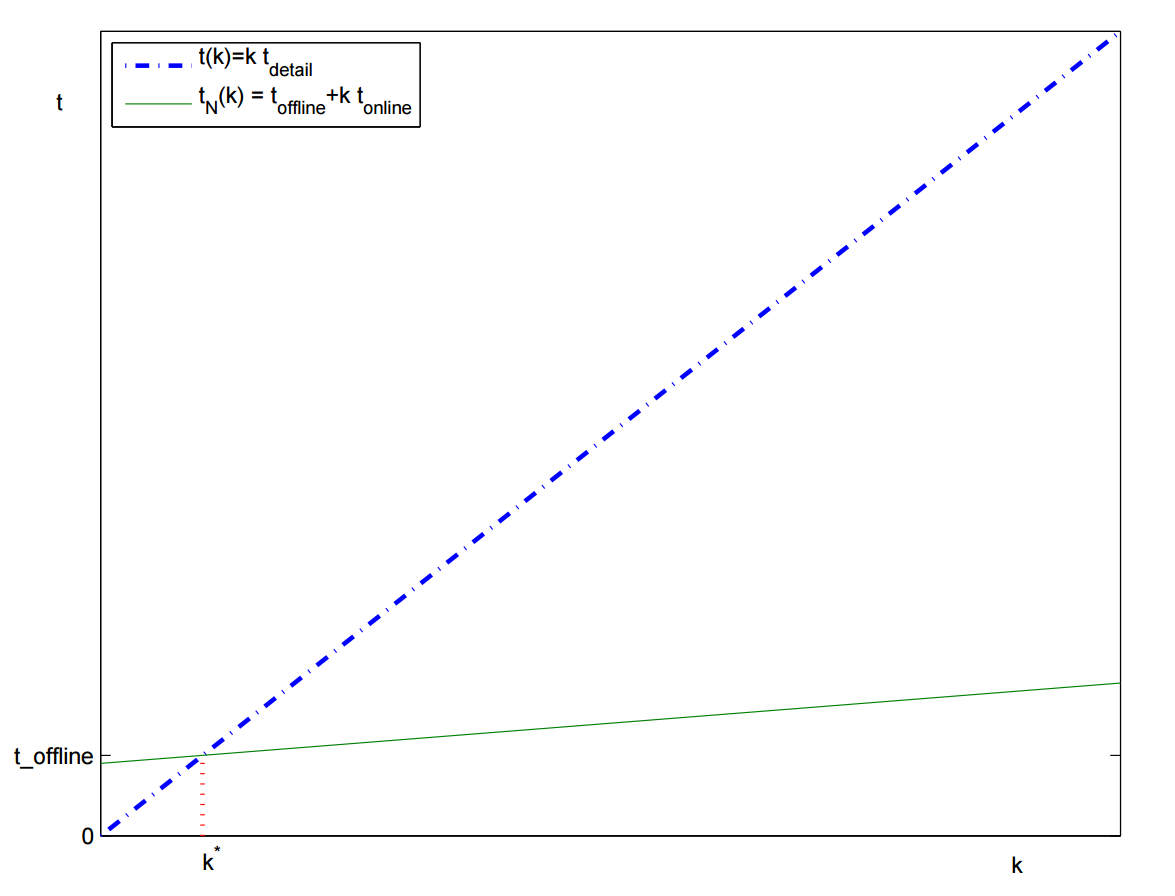
\includegraphics[width = 0.5 \textwidth]{Bilder/Laufzeiten.png}
		\caption{Laufzeiten mit wachsender Anzahl an Simulationen.}{(aus B. Haasdonk, Reduzierte-Basis-Methoden, Skript zur Vorlesung SS 2011, Universität Stuttgart, IANS-Report 4/11, 2011.)}
		\label{fig:Laufzeiten}
	\end{figure}
	\end{itemize}
\end{bem}

\begin{bem}[Keine Unterscheidung zwischen $u$ und $u_h$]
	Erinnerung: Wir unterscheiden (meistens) nicht in Notation zwischen $u_h$ (FEM-Lösung) und $u$ (Sobolev-Raum Lösung). Dies kann nun begründet werden:
	\begin{enumerate}
		\item Die Online-Phase ist unabhängig von $H = \dim(X)$, daher kann $H$ beliebig groß und damit $u_h$ beliebig präzise gemacht werden durch geeignete Diskretisierung mit genügend feinem Gitter, so dass $u$ und $u_h$ praktisch ununterscheidbar sind ($||u - u_h ||$ beliebig klein aber $(P_N(\mu))$ schnell lösbar).
		\item In der Praxis wird Reduktionsfehler den Gesamtfehler dominieren, der (FEM-)Diskretisierungsfehler spielt untergeordnete Rolle.
		\[
			\epsilon := ||u - u_h|| \ll ||u_h - u_N||
		\]
		\[
			\Rightarrow ||u_h - u_N|| - \epsilon \leq \underbrace{||u-u_N||}_{\text{theoretisch das Ideal}} \leq \overbrace{||u_h - u_N||}^{\text{berechenbar}} + \epsilon
		\]
		also kontrollieren wir durch Fehlerschranken für $||u_h - u_N||$ bis auf $\epsilon$ auch den eigentlich interessanten Fehler $||u - u_N||$.
	\end{enumerate}
\end{bem}

\subsection{Offline-/Online- Zerlegung für Fehlerschranken/Effektivitätsschranken}

Für schnelle Berechnung der Fehlerschranken \& Effektivitätsschranken benötigen wir Zerlegung für
\begin{itemize}
	\item Duale Norm des Residuums $|| r(\pdot ; \mu)||_{X'} = ||v_r||$ für alle Fehlerschranken
	\item Duale Norm des Ausgabefunktionals $|| l(\pdot;\mu)||_{X'}$ für $\Delta_{N,s}(\mu)$
	\item Norm $||u_N (\mu) ||_X$ der RB-Lösung für relativen Energienormfehlerschätzer $\Delta_N^{en, rel}$.
	\item Untere/obere Schranke $\alpha_{LB}(\mu)$ bzw. $\gamma_{UB} (\mu)$ für Koerzivitäts- bzw. Stetigkeitskonstante für Fehlerschätzer bzw. Effektivitätsschranken.
\end{itemize}
Separierbarkeit von $(P(\mu))$ überträgt sich auf Residuum

\begin{satz}[Separierbare Parameter-Abhängigkeit für $r(\pdot;\mu)$]
\label{3.22}
	Seien $a, f$ sep. parametrisch. Nach Riesz existieren $v_f^q \in X$ mit $<v_f^q, v> = f^q(v) \,\,\, \forall v \in X, \, q=1,...,Q_f$ und $v_a^{q,n} \in X$ mit $<v_a^{q,n}, v> = a^q (\phi_n,v), \, v \in X, \, q=1,...,Q_a, n=1,...,N$
	Setze $Q_r := N Q_a + Q_f$ und Aufzählung von $\{v_a^{q,n},v_f\}$ durch
	\[
		(v_r^1,...,v_r^{Q_r}) := (v_f^1,...,v_f^{Q_f},v_a^{1,1},...,v_a^{Q_a,1},v_a^{1,2},...,v_a^{Q_a,2},...,v_a^{Q_a,N})
	\]
	Für $\mu \in \mathcal{P}$ sei $u_N = \sum_{n=1}^N u_{Nn} \phi_n$ Lösung von $(P_N(\mu))$ und hiermit definiere
	\begin{align*}
		(\Theta_r^1(\mu),...,\Theta_r^{Q_r}(\mu)) := (\Theta_f^1(\mu),...,\Theta_f^{Q_f}(\mu),-\Theta_a^{1}(\mu),...,-\Theta_a^{Q_a}(\mu)u_{N1},-\Theta_a^{1}(\mu)u_{N2},... \\
		...,-\Theta_a^{Q_a}(\mu)u_{N2},...,-\Theta_a^{Q_a}(\mu)u_{NN})
	\end{align*}
	Mit $r^q(\pdot) := <v_r^q, \pdot> \in X', \, q = 1,...,Q_r$ sind $r(\pdot;\mu)$ und $v_r(\mu)$ separierbar parametrisch via
	\[
		r(\pdot;\mu) = \sum_{q=1}^{Q_r} \Theta_r^{q}(\mu) \cdot r^q(\pdot), \qquad v_r(\mu) = \sum_{q=1}^{Q_r} \Theta_r^{q}(\mu) \cdot v_r^q \qquad \forall \mu \in \mathcal{P}
	\]
\end{satz}

\begin{proof}
	Definition und Linearität ergibt:
	\begin{align*}
		<v_r(\mu),v> = r(v;\mu) &= f(v;\mu) - a(u_N(\mu),v;\mu) \\
		&= \sum_q \Theta_f^q(\mu) f^q (v) - \sum_q \sum_n \Theta_a^q (\mu) u_{Nn} a^q(\phi_n,v) \\
		&= \underbrace{<\sum_q \Theta_f^q (\mu) v_f^q - \sum_q \sum_n \Theta_a^q (\mu) u_{Nn} v_a^q, v>}_{\sum \Theta_r^q (\mu) v_r^q} \\
		&= \sum_{q=1}^{Q_r} \Theta_r^q (\mu) r^q(v) \qquad \forall v \in X
		\label{eq:3.5}
	\end{align*}
\end{proof}

Offensichtlich Berechnung von Riesz-Repräsentant notwendig, dies geschieht durch Ausnutzen der Endlichdim. von $X = \op{span}\{\psi_i\}_{i=1}^Ĥ$ und $K := (<\psi_i,\psi_j>)_{i,j=1}^H$

\begin{satz}[Berechnung von Riesz-Repr.]
	Für $g \in X'$ erhält man Koeffizientenvektor $\underbar v = (v_i)_{i=1}^H \in \R^H$ seines Riesz-Repräsentanten $v_g = \sum_{i=1}^H v_i \, \psi_i \in X$ durch lösen von
	\begin{align}
		K \underbar v = \underline{g}
	\end{align}
	mit Vektor $\underline{g} := (g(\psi_i))_{i=1}^H \in \R^H$
\end{satz}

\begin{proof}
	Für jedes $u = \sum_{i=1}^H u_i \, \psi_i \in X$ mit Koeffizientenvektor $\underbar u = (u_i)_{i=1}^H$ erhalten wir
	\[
		g(u) = g(\sum u_i \, \psi_i) = \sum u_i \, g(\psi_i) = \underbar u^T \underline{g} \overset{\ref{eq:3.5}}{=} \underbar u^T K \underbar v = <u,v_g>
	\] 
\end{proof}

\begin{bem}
	\ref{eq:3.5} ist typischerweise dünn besetzt, also mit iterativen LGS-Lösern berechenbar.
\end{bem}

\begin{kor}[Offline-/Online- für Residuen-Norm]
\label{3.24}
	(Offline:) Nach Offline von $(P_N(\mu))$ gemäß \ref{3.21} def. $G_r := <r^q (v_r^{q'})>_{q,q' =1}^{Q_r} \in \R^{Q_r \times Q_r}$ mittels Residuen-Komponenten $r^q$ und Riesz-Repr. $v_r^q$ aus \ref{3.22}
	(Online:) Für $\mu \in \mathcal{P}$ und RB-Lösung $\underbar u_N \in \R^N$ berechne Residuen-Koeff-Vektor $\underline{\Theta}_r(\mu) = (\Theta_r^1(\mu),...,\Theta_r^{Q_r} (\mu))^T \, \in \R^{Q_r}$.
	Dann gilt: 
	\begin{align}
	||v_r(\mu)||_X = ||r(\pdot;\mu)||_X = \sqrt{\underline{\Theta}_r(\mu)^T \cdot G_r \underline{\Theta}_r(\mu)}
	\label{eq:3.6}
	\end{align}
\end{kor}

\begin{proof}
	Zunächst sehen wir $G_r = (<v_r^q,v_r^{q'}>)_{q, q' = 1}^{Q_r}$. Isometrie der Riesz-Abbildung \& Separierbarkeit ergeben
	\[
		||r(\mu)||_X^2 = ||v_r(\mu)||_X^2 = <\sum_{q=1}^{Q_r} \Theta_r^q(\mu) \, v_r^q,\sum_{q'=1}^{Q_r} \Theta_r^{q'}(\mu) \, v_r^{q'}>= \underline{\Theta}_r^T \cdot G_r \cdot \underline{\Theta}_r (\mu) 
	\]
\end{proof}

\begin{bem}[Stabilisierung durch Orthonormierung von $\{v_r^q\}$]
	Wie in \textsf{demos\_chapter3(3)} gesehen, existiert eine Genauigkeitsgrenze für Fehlerschätzer, diese liegt in numerischen Auslöschungseffekten in \ref{eq:3.6} begründet, denn $G_r$ ist potentiell schlecht konditioniert. Gemäß einer Idee von Behr \& Rave 2014 lässt sich die Genauigkeit steigern, indem die $\{v_r^q\}$ orthonormiert werden und \ref{eq:3.6} mit entsprechender Transformationsmatrix modifiziert werden.
\end{bem}

\begin{kor}[Offline-/Online- Zerlegung für $||l(\pdot;\mu)||_{X'}$]
	(Offline:) Berechne Riesz-Repr. $v_l^q \in X$ der Ausgabekommponenten, d.\,h.
	\[
		<v_l^q,v> = l^q(v) \qquad \forall v \in X, \, q=1,...,Q_l
	\]
	und def. $G_l := (l^q(v_l^{q'})_{q, q' =1}^{Q_l}$
	(Online:) Zu $\mu \in \mathcal{P}$ berechne $\underline{\Theta}_l (\mu) := (\Theta_l^1(\mu),...,\Theta_l^{Q_l}(\mu))$ und $||l(\pdot;\mu)||_{X'} = \sqrt{\underline{\Theta}_l^T G_l \underline{\Theta}_l}$
\end{kor}

\begin{proof}
	analog zu \ref{3.24}
\end{proof}

\begin{kor}[Offline-/Online für $||u_N(\mu)||_X,\, ||u_N(\mu)||_{\mu}$]
	(Offline:) Nach der Offline-Phase von $(P_N(\mu))$ def.
	\[
		K_N := (<(\phi_i,\phi_j>)_{i,j=1}^N \, \in \R^{N \times N}
	\]
	(Online:) Zu $\mu \in \mathcal{P}$ berechne $A_N(\mu)$ und $\underbar u_N(\mu)$ durch Online-Phase von $(P_N(\mu)$
	\[
		|| u_N(\mu)||_X = \sqrt{\underbar u_N^T \, K_N \, \underbar u_N}
	\]
	\[
		|| u_N(\mu)||_{\mu} = \sqrt{\underbar u_N^T \, (\frac{1}{2} (A_N(\mu) + A_N(\mu)^T)) \, \underbar u_N}
	\]
\end{kor}

\begin{proof}
	\begin{align*}
		||u_N||^2 = <\sum_n u_{Nn} \phi_n \, , \, \sum u_{Nn'} \phi_{n'}> = \sum_{n, n'} u_{Nn} u_{Nn'} <\phi_n, \phi_{n'}> = \underbar u_N^T \cdot K_N \cdot \underbar u_N
	\end{align*}	
	analog für Energienorm mit $A_{N,s} := \frac{1}{2} (A_N(\mu) + A_N(\mu)^T)$
\end{proof}

\begin{bem}
	$K_N$ wieder einfach aus $K$ berechenbar (Übung).
\end{bem}

Für Fehlerschranken fehlen noch untere Schranke $\alpha_{LB} (\mu) \le \alpha (\mu)$, welche schnell berechenbar sein sollen.
Falls $a(\pdot , \pdot ; \mu)$ glm. koerziv bzgl. $\mu$ und $\bar{\alpha} < 0$ bekannt, so ist $\alpha_{LB} (\mu) := \bar{\alpha}$ gültige Wahlmöglichkeit.
In gewissen Fällen kann eine größere und damit bessere Schranke angegeben werden.

\begin{satz}[``Min-$\Theta$-Verfahren'' zur Berechnung von $\alpha_{LB}(\mu)$]
	Seien $a^q(u,u) \geq 0 \,\, \forall q,u$ und $\Theta_a^q (\mu) > 0 \,\, \forall \mu$ \\
	(Offline:) Sei $\alpha(\bar{\mu})$ für ein $\bar{\mu} \in \mathcal{P}$ verfügbar \\
	(Online:) Setze für $\mu \in \mathcal{P}$
	\[
		\alpha_{LB} (\mu) := \alpha(\bar{\mu}) \cdot \min_{q} \frac{\Theta_a^q(\mu)}{\Theta_a^q(\bar{\mu})}
	\]
	Dann gilt $0 < \alpha_{LB} (\mu) \leq \alpha(\mu)$
\end{satz}

\begin{proof}
	Wegen $0 < \alpha(\bar{\mu})$ und $0 < c(\mu) := \min\limits_q \frac{\Theta_a^q(\mu)}{\Theta_a^q(\bar{\mu})}$ gilt $ 0 < \alpha(\bar{\mu}) \cdot c(\mu) := \alpha_{LB}(\mu)$
	Folgende Argumentation ähnlich zu \ref{2.6} ii) \\
	Für alle $u \in X$ gilt
	\begin{align*}
		a(u,u;\mu) &= \sum\limits_q \Theta_a^q(\mu) \, a^q(u,u) = \sum\limits_q \frac{\Theta_a^q(\mu)}{\Theta_a^q(\bar{\mu})} \cdot \Theta_a^q(\bar{\mu}) \, a^q(u,u) \\
		&\geq \sum\limits_q \underbrace{\Bigl( \min\limits_{q'} \frac{\Theta_a^{q'}(\mu)}{\Theta_a^{q'}(\bar{\mu})} \Bigr)}_{c(\mu)} \cdot \Theta_a^q(\bar{\mu}) \, a^q(u,u) \\
		&= c(\mu) \cdot \underbrace{\sum\limits_q \Theta_a^q(\bar{\mu}) \, a^q(u,u)}_{= a(u,u;\bar{\mu})} = c(\mu) \, a(u,u;\bar{\mu}) \\
		&\overset{\text{glm. koerziv bzgl} \mu}{\geq} c(\mu) \cdot \alpha(\bar{\mu}) \cdot ||u||^2 \\
		&= \alpha_{LB}(\mu) \cdot ||u||^2
	\end{align*}
	Also insbesondere
	\[
		\alpha(\mu) = \inf\limits_u \frac{a(u,u;\mu)}{||u||^2} \geq \alpha_{LB}(\mu)
	\]
\end{proof}

\begin{bem} \beginwithlistbem
	\begin{itemize}
		\item ``Min-$\Theta$'' kann für Thermischen Block angewandt werden
		\item obiges gilt auch für nichtsymm. $a(\pdot , \pdot)$
		\item $\alpha(\bar{\mu})$ kann mittels eines hochdimensionalen Eigenwertproblems bestimmt werden:
	\end{itemize}
\end{bem}

\begin{satz}[Berechnung von $\alpha(\mu)$ für $(P(\mu))$]
	Seien $A(\mu), \, K \in \R^{H \times H}$ wie in \ref{3.19}/\ref{3.20}. \\
	Setze $A_s(\mu) := \frac{1}{2} (A(\mu) + A(\mu)^T)$. Dann gilt
	\[
		\alpha(\mu) = \lambda_{\op{min}} (K^{-1} A_s(\mu))
	\]
	wobei $\lambda_{\op{min}}$ den kleinsten Eigenwert bezeichnet.
\end{satz}

\begin{proof}
	Sie $K = L L^T$ (z.\,B. Cholesky oder Matrix-Wurzel) und verwende $\underbar v = L^t \underbar u$:
	\begin{align*}
		\alpha (\mu) &= \inf\limits_{u \in X} \frac{a(u,u;\mu)}{||u||^2} = \inf\limits_{\underbar u \in \R^H} \frac{\underbar u^T A(\mu) \underbar u}{\underbar u^T K \underbar u} \\
		&= \inf\limits_{\underbar u \in \R^H} \frac{\underbar u^T A_s(\mu) \underbar u}{\underbar u^T K \underbar u} \\
		&= \inf\limits_{\underbar v \in \R^H} \frac{\underbar v^T L^{-1} A_s \overbrace{L^{-T}}^{\text{inv. transp.} -1 \cdot T} \underbar v}{\underbar v^T L^{-1} L L^T L^{-T} \underbar v} = \inf\limits_{\underbar v \in \R^H} \frac{\underbar v^T L^{-1} A_s L^{-T} \underbar v}{\underbar v^T \underbar v}
	\end{align*}
	Also ist $\alpha(\mu)$ Minimum eines Rayleigh-Quotionenten, also kleinster Eigenwert der symmetrischen \& positiv definiten Matrix $\bar{A_s} := L^{-1} A_s L^{-T}$ \\
	Die Matrizen $\bar{A_s}$ und $K^{-1} A_s$ sind ähnlich, da 
	\[
		L^T(K^{-1}A_s)L^{-T} = L^T L^{-T}L^{-1}A_sL^{-T} = L^{-1}A_sL^{-T} = \bar{A_s}
	\]
	Also haben sie identische Eigenwerte.
\end{proof}

\begin{bem} \beginwithlistbem
	\begin{itemize}
		\item Inversion von $K$ muss verhindert werden. Daher verwende EW-Löser, welcher nur Matrix-Vektor-Multiplikation verwendet. Sobald ein Produkt $y=K^{-1}A_s x$ erforderlich ist, löst man das System $Ky = A_s x$. Alternativ kann auch kleinster EW eines verallgemeinerten EWP $A_s \underbar u = \lambda K \underbar u$ berechnet werden.
		\item Für variationelle Form des verallg. EWP für $\infty$-dim $(P(\mu))$ siehe Patera \& Rozza
		\item Für Probleme, bei denen die Voraussetzungen von Min-$\Theta$ nicht erfüllt sind, kann ``Successive Constraint Method'' (SCM) eine Alternative darstellen.  $\leadsto$ §\ref{sec-4}
	\end{itemize}
\end{bem}

\begin{satz}[``Max-$\Theta$''-Verfahren für $\gamma_{UB}(\mu)$, symmetrisches $a(\pdot , \pdot)$]
	Sei $a$ symmetrisch, koerziv, separierbar parametrisch mit $a^q$ positiv semidefinit und $\Theta_a^q > 0 \, \, \forall q,u$ \\
	(Offline:) Sei $\bar{\mu} \in \mathcal{P}$ und $\gamma(\bar{\mu})$ berechnet \\
	(Online:) Setze für $\mu \ in \mathcal{P}: \gamma_{UB}(\mu) := \gamma(\bar{\mu}) \max\limits_q \frac{\Theta_a^q(\mu)}{\Theta_a^q(\bar{\mu})}$. Dann gilt 
	\[
		\gamma_{UB}(\mu) \leq \gamma_{UB} (\mu) < \infty
	\]
\end{satz}

\begin{proof}
	Übung.
\end{proof}

\begin{bem}[Komplexitäten]
	Durch die angegebenen Berechnungsverfahren ist vollständige Offline-/Online-Zerlegung der RB-Lösung, Fehlerschranken und Effektivitätsschranken erreicht (Offline unabh. von $\mu$, Online unabh. von $H$). Komplexitäten für $\Delta_N(\mu), \Delta_{N,s}(\mu)$:
	\begin{itemize}
		\item Offline: $\O(H^3 + H^2 (Q_f + Q_l + N Q_a) + H Q_l^2 + H(Q_f + NQ_a)^2$ für EWP für $\alpha(\bar{\mu})$,
			Riesz-Repräsentanten für $f^q$, $l^q$, $a^q(\phi_n,\pdot)$ und Matrix $G_l$ und $G_r$
		\item Online: $\O((Q_f+N Q_a)^2 + Q_l^2 + Q_a)$ für Berechnung von $\norm{v_r(\pdot;\mu)}$, $\norm{l(\pdot;\mu)}_{X'}$ und $\alpha_{LB}(\mu)$ durch Min-$\Theta$.
			Problematisch ist quadratische Abhängigkeit von $Q_f$, $Q_l$, $N Q_a$, welches diese Größen in der Praxis stark einschränkt.
	\end{itemize}
\end{bem}

\paragraph{demos\_chapter3(4)} Beispiel-Lauf von Reduktionsschritten in RBmatlab.

\subsection{Basisgenerierung}
\label{sec-3.4}

\subsubsection*{Approximation durch lineare Unterräume}

Motivation für Snapshot-basierte Verfahren:
\begin{itemize}
	\item Bestimmung eines möglichst guten $X_N$, welches $\LM$ global approximiert.
	\item Formulierung durch Optimierungsproblem, z.B.\ minimiere maximalen Fehler in Energienorm
		\begin{equation}
			\min_{\stackrel{Y \subset X}{\dim Y = N}} \max_{\mu \in \p} \norm{u(\mu)-u_N(\mu)}_\mu
		\end{equation}
		oder Minimum des mittleren quadratischen Projektionsfehlers
		\begin{equation}
			\min_{\stackrel{Y \subset X}{\dim Y = N}} \int_\p \norm{u(\mu)-P_Y u(\mu)}^2 \,\mathrm{d}\mu
		\end{equation}
		oder beliebiges anderes Distanzmaß.
\end{itemize}
